\documentclass[12pt,a4paper,titlepage,oneside]{report}

%%{{{ packages
%% font encoding.
\usepackage[utf8]{inputenc}
\usepackage[T1]{fontenc}
\usepackage{lmodern}
\usepackage{couriers}
%% Customize chapters.
\usepackage{titlesec}
%% bibliography.
\usepackage[backend=bibtex,style=ieee]{biblatex}
%% \includegraphics{name}
\usepackage{graphicx}
%% \url{something}
\usepackage{url}
%% \multirow{package}{width}{text}
\usepackage{multirow}
%% \cellcolor
\usepackage[table]{xcolor}
%% \caption{title}
\usepackage{caption}
\usepackage{subcaption}
%% \forloop
\usepackage{forloop}
%% fix underfull on footnote with URL.
\usepackage{ragged2e}
%% source code listing
\usepackage{listings}
%% \printindex
\usepackage{makeidx}
%% table of content
\usepackage{tocloft}
%% text emphasis, including strikeout.
\usepackage[normalem]{ulem}
%% mathematics
\usepackage{mathtools}
%% arithmetic
\usepackage{calc}
%% algorithm
\usepackage{algorithm}
\usepackage{algpseudocode}
%% multiple columns
\usepackage{multicol}
%% Change the margin
\usepackage[a4paper]{geometry}
\geometry{
	a4paper,
	top=3cm,
	right=3cm,
	bottom=3cm,
	left=4cm
}
%%
\usepackage{parskip}
%% Package for reading CSV to database.
\usepackage{datatool}
%% Package for scatter and line plot.
\usepackage{dataplot}
%% Long table
\usepackage{longtable}
%% Tikz
\usepackage{pgfplots}

%% Add box to figure.
%%
\usepackage{float}

\floatstyle{boxed}
\restylefloat{figure}

%% MnSymbol
\usepackage{MnSymbol}
%%}}}

%%{{{ hyphenation: sorted in ascending.
%%
\hyphenation{
	Ja-nu-a-ri
	SIGKDD
	Wiki-pedia
	a-kan
	ang-ka
	ba-gai-ma-na
	bayes-ian
	ber-kas
	ber-ma-sa-lah
	ber-mak-na
	bi-a-ya
	da-lam
	data-set
	de-ngan
	di-ha-sil-kan
	di-sing-kat
	di-tam-bah-kan
	dis-krit
	fung-si
	ga-bung-an
	ke-las
	ke-mung-ki-nan
	ke-tak-se-imbang-an
	lan-guage
	ma-yo-ri-tas
	me-laku-kan
	me-me-rik-sa
	me-mi-lih
	me-ne-rap-kan
	me-ning-kat-kan
	me-nye-dia-kan
	me-nye-im-bang-kan
	me-sin
	me-thod
	mem-vi-sua-li-sa-si
	meng-gu-na-kan
	meng-hu-bung-kan
	meng-i-kut-kan
	meng-i-kuti
	meng-im-ple-men-ta-si-kan
	meng-in-di-ka-si-kan
	mi-sal-nya
	mung-kin
	o-ver-sam-pling
	pa-ra-lel
	pe-mi-sah
	pe-nan-da
	pe-ne-li-ti-an
	pe-nu-li-san
	pe-nyun-ting
	pem-ban-ding
	pen-de-kat-an
	peng-kla-si-fi-ka-si
	per-for-man-si-nya
	po-ten-si-al
	pro-ba-bi-li-tas
	pro-ses
	sam-pel
	se-im-bang
	se-jum-lah
	sun-ting-an
	ting-kat
	un-der-sam-pling
	wa-lau-pun
}
%%}}}

%%{{{ override default latex setting.
%%

%% Space between paragraphs.
\setlength{\parskip}{1.5em}

%% Add dot to TOC.
\renewcommand{\cftsecleader}{\cftdotfill{\cftdotsep}}
\renewcommand{\contentsname}{}

\lstset{
	basicstyle=\scriptsize\ttfamily
,	breaklines=true
,	stringstyle=\scriptsize\ttfamily
,	numbers=left
,	numberstyle=\tiny\ttfamily
,	numbersep=5pt
,	tabsize=4
,	frame=single
}

\makeatletter
\def\lst@lettertrue{\let\lst@ifletter\iffalse}
\makeatother

%% Format chapter and section.
%%
%%% Set chapter name to Bab.
\titleformat{\chapter}[hang]
{\bfseries\large\centering}
{Bab \thechapter}
{1em}
{}

\titleformat{\section}[hang]
{\bfseries\large}
{\thesection}
{1em}{}

%% Set spacing for sections.
\titlespacing{\chapter}{0ex}{0ex}{1.5em}
\titlespacing{\section}{0ex}{0ex}{0em}

%% Alter latex default title on table.
\captionsetup[table]{name=Tabel}
\captionsetup[figure]{name=Gambar}

\renewcommand{\arraystretch}{1.5}
\setlength{\tabcolsep}{3pt}

%% Change bibliography title.
\defbibheading{bibliography}{\centerline{
	\textbf{DAFTAR REFERENSI}}
}

%%% uncomment this to show overrule in black box
\overfullrule=2cm

%% Algorithmicx
\makeatletter
\renewcommand{\ALG@beginalgorithmic}{\footnotesize}
\makeatother

%% multicolumn setting
\setlength{\columnsep}{1cm}

%% pgfplots setting.
\pgfplotsset{
	/pgf/number format/read comma as period,
	/pgf/text mark as node=false,
	table/col sep=semicolon,
	xmax=1,
	xmin=0,
	ymax=1,
	ymin=0,
	xtick distance=0.2,
	ytick distance=0.2,
	grid=major,
	cycle list name=linestyles,
}
%%}}}

%%{{{ variables
%%
\newcommand{\mytitle}{Deteksi Vandalisme pada Wikipedia Bahasa Inggris menggunakan klasifikasi Cascaded Random Forest}
\newcommand{\myname}{Muhamad Sulhan}
\newcommand{\mysid}{23513014}
\newcommand{\myadvisorname}{Dwi Hendratmo Widyantoro}
\newcommand{\myadvisorid}{196812071994021001}
\newcommand{\mydept}{Program Studi Magister Informatika}
\newcommand{\itb}{Institut Teknologi Bandung}

%%% My images directory
\graphicspath{{../images/}}
\newcommand{\myitbcover}{ITB-logo-hitam}

%%% My bibligraphy file
\addbibresource{bibliography.bib}
%%}}}

%%{{{ document's meta-data
%%
\author{\myname}
\title{\mytitle}
%%}}}

%%{{{ document's macros
%%
%%% two column signature.
\def\myadvisorsig#1{%
	\vbox{\hsize=6cm
		\textbf{#1}\\
		\addvspace{2cm}%
		\hbox to \hsize{%
			\strut\hfil%
			\myadvisorname%
			\hfil%
		}
		\hrule\kern1ex
		\hbox to \hsize{%
			\strut\hfil%
			NIP\hspace{1ex}\myadvisorid%
			\hfil%
		}
	}
}

%%% one column signature.
\def\mysignature#1#2#3{%
	\vbox{
		\textbf{#1}\\
		\addvspace{2cm}%
		\hbox to \hsize{%
			\strut\hfil%
			{#2}%
			\hfil%
		}
		\makebox[6cm][c]{
			\hrulefill
		}
		\hbox to \hsize{%
			\strut\hfil%
			NIP\hspace{1ex}{#3}%
			\hfil%
		}
	}
}

%%% source code listing
\lstdefinelanguage{go}
{
	morekeywords={package,import,const,func,for,type,var,struct}
,	sensitive=true
,	morecomment=[l]{//}
,	morecomment=[s]{/*}{*/}
}
\lstdefinestyle{go}{%
	language=go
,	keywordstyle=\color{black}\bfseries
,	commentstyle=\color{gray}
,	breakatwhitespace=true
,	lineskip={-2.5pt}
}
\newcommand{\includecodego}[2][c]{
	\lstinputlisting[caption=#2,escapechar=,style=go]
		{/home/ms/go/work/src/github.com/shuLhan/#2}
}

%%% data listing
\lstdefinestyle{data}{%
	breakatwhitespace=false
,	breakautoindent=false
,	literate={\,}{}{0\discretionary{,}{}{,}},
}
\newcommand{\includedata}[2][c]{
	\lstinputlisting[caption=#2,style=data,linerange={1-10}]
		{/home/ms/go/work/src/github.com/shuLhan/#2}
}
%%}}}


\begin{document}

\thispagestyle{empty}
\begin{center}
\textbf{\large
	\MakeUppercase{\judul} \\
	\vfill
	TESIS \\
	\bigskip
	{\normalsize
		Karya tulis sebagai salah satu syarat \\
		untuk memperoleh gelar Magister dari \\
		\itb{} \\
	}
	\vfill
	{\normalsize Oleh} \\
	\MakeUppercase{\myname{}} \\
	NIM: \mysid{} \\
	\mydept{} \\
	\vfill
	\includegraphics[width=2.35cm,height=3.5cm]{\myitbcover} \\
	\vfill
	\normalsize
	\MakeUppercase{\tfakultas} \\
	\MakeUppercase{\itb{}} \\
	Mei 2016 \\
}
\end{center}


\newpage
\pagenumbering{roman}
\begin{center}
\textbf{\large
	\MakeUppercase{\mytitle{}} \\
	\bigskip
	\textnormal{Oleh} \\
	\myname{} \\
	NIM: \mysid{} \\
	(\mydept{}) \\
}
\end{center}

\bigskip
\bigskip
\bigskip

Wikipedia.org adalah ensiklopedia daring yang dapat disunting oleh siapa saja.
Sifat wiki ini dapat mempercepat perbaikan dan pertumbuhan artikel,
kekurangannya yaitu dapat menimbulkan vandalisme dalam bentuk suntingan dengan
informasi yang salah, penghapusan, iklan, atau teks yang tidak bermakna.
Tesis ini membahas deteksi vandalisme menggunakan pembelajaran mesin
dengan menerapkan metode klasifikasi
\textit{Cascaded Random Forest} (CRF)
yang dilatih pada dataset
\textit{Wikipedia Vandalism Corpus 2010}
yang telah
disampel ulang dengan
\textit{Local Neighbourhood Synthetic Minority Over-sampling Technique}
(LNSMOTE).
Kedua metode tersebut dibandingkan dengan klasifikasi
\textit{Random Forest} (RF)
dan teknik sampel ulang SMOTE.
Hasil sampel ulang dan pemodelan diuji dengan dataset
\textit{Wikipedia Vandalism Corpus 2011}
menunjukan hasil sampel ulang dengan LNSMOTE meningkatkan laju
\textit{true-positive} lebih tinggi daripada dataset yang tidak disampel ulang
dan yang disampel ulang dengan SMOTE pada kedua pengklasifikasi.
Dari segi performansi, CRF dengan sampel ulang LNSMOTE dengan 200 tingkat dan 1
pohon memberikan hasil yang paling baik dengan nilai TPR yaitu $0,9904$.
Dari segi kecepatan pemodelan pengklasifikasi CRF lebih cepat 1,6 kali daripada
RF pada data yang telah disampel ulang.

Kata kunci: wikipedia, vandalisme, dataset timpang, dataset sampel ulang,
\textit{cascaded random forest}


\newpage
\pagenumbering{arabic}

\chapter{Pendahuluan}

\section{Latar Belakang}
\label{sec:latar-belakang}

Wikipedia.org adalah ensiklopedia daring dan terbuka, yang mana artikel di
Wikipedia merupakan hasil kolaborasi para penyunting dari seluruh dunia.
Terbuka artinya siapa pun dapat menyunting artikel tanpa perlu melakukan
registrasi terlebih dahulu.
Ensiklopedia daring ini memiliki artikel dari berbagai bahasa, dari bahasa umum
dunia seperti Bahasa Inggris, sampai bahasa daerah seperti Bahasa Jawa.

Vandalisme menurut Kamus Besar Bahasa Indonesia daring adalah,
1) perbuatan merusak dan menghancurkan hasil karya seni dan barang berharga
lainnya;
2) perusakan dan penghancuran secara kasar dan ganas.
Dalam konteks Wikipedia.org, vandalisme dapat berbentuk suntingan yang mengubah
konten dari artikel sehingga memberikan isi yang salah, penghapusan secara
menyeluruh, penghapusan sebagian, isi yang menghina, iklan, dan/atau teks yang
tidak ada maknanya.

Jumlah artikel Bahasa Inggris pada situs en.wikipedia.org pada bulan Juli 2015
yaitu sebanyak 4,932,627 artikel, dengan pengguna aktif, atau disebut juga
penyunting, sebanyak 31,369 orang.
Berarti, jika diasumsikan semua penyunting benar aktif, maka setiap pengguna
aktif harus mengawasi kurang lebih 157 artikel.
Menemukan dan memperbaiki vandalisme tersebut dapat mengganggu penyunting dari
menulis artikel dan pekerjaan penting lainnya, dan membuat pembaca bisa
mendapatkan informasi yang salah atau tidak mendapatkan informasi sama sekali.


\section{Rumusan Masalah}
\label{sec:rumusan-masalah}

Korpus yang umum digunakan untuk pembelajaran vandalisme pada Wikipedia yaitu
\textit{PAN Wikipedia Vandalism Corpus} 2010 (PAN-WVC-10)
\cite{potthast:2010b}
atau
\textit{PAN Wikipedia Vandalism Corpus} 2011 (PAN-WVC-11)
\cite{potthast:2010b}
dengan tingkat bias yang tinggi pada data.
Kedua korpus tersebut memiliki jumlah yang tidak seimbang antara suntingan
biasa dengan jumlah suntingan vandal.
PAN-WVC-10 untuk artikel Wikipedia bahasa Inggris memiliki 32.439 sampel dengan
2394, atau 7\%, diantaranya adalah vandal, sedangkan korpus PAN-WVC-11 untuk
artikel Wikipedia bahasa Inggris memiliki jumlah 9985 suntingan dengan 1144,
atau 8\%, diantaranya adalah vandal.

\newpage
Menerapkan klasifikasi dengan dataset yang bias bisa menyebabkan performansi
deteksi yang rendah.
Hal ini bisa disebabkan oleh,
\begin{enumerate}
	\item Jika sebuah klasifikasi belajar dengan meminimalkan keseluruhan
	galat, maka instan dari kelas yang minoritas memiliki kontribusi yang
	rendah terhadap galat.
	Hal ini menyebabkan bias yang condong pada kelas klasifikasi yang
	mayoritas.
	\item Pada umumnya klasifikasi mengasumsikan distribusi kelas yang
	seimbang antara kelas minoritas dan mayoritas, yang terkadang pada
	dunia nyata kasusnya tidak selalu seperti itu.
	\item Sering kali klasifikasi secara implisit mengasumsikan biaya yang
	sama untuk mis-klasifikasi pada kedua kelas tersebut, yang mana
	terkadang tidak masuk akal.
	Sebagai contohnya, biaya untuk mengklasifikasikan kanker sebagai bukan
	kanker lebih tinggi dari pada sebaliknya.
	Secara tidak adanya data kanker bisa menyebabkan tidak dilakukannya
	terapi, misklasifikasi bisa membahayakan nyawa.
\end{enumerate}

Untuk mengatasi masalah ketimpangan pada korpus, Gotze
\cite{gotze2014advanced}
mengaplikasikan teknik
\textit{random undersampling}
bernama
\textit{Synthetic Minority Over-sampling TEchnique} (SMOTE)
yang diajukan oleh Chawla
\cite{chawla2002smote},
dan kombinasi dari SMOTE dan
\textit{random undersampling}.
Dataset latihan yang orisinal dan hasil sampel ulang diuji dengan
pengklasifikasi satu-kelas dan dua-kelas.
Pengklasifikasi satu-kelas yang diterapkan diantaranya Hempstalk dkk.
\cite{hempstalk2008one}
dan SVM oleh Schölkopf dkk.
\cite{scholkopf1999support}
yang diimplementasikan oleh Chang dan Lin
\cite{chang2011libsvm}
pada korpus PAN-WVC.
Pengklasifikasi dua-kelas yang diterapkan diantaranya
\textit{Logistic Regression},
\textit{RealAdaBoost},
\textit{Random Forest} (RF), dan
\textit{Bayesian Network}.
Hasil percobaan yang didapat memperlihatkan performansi pengklasifikasi
satu-kelas tidak kompetitif dengan satu pun pengklasifikasi dua-kelas.
Hal ini bisa disebabkan karena tidak sesuainya kelompok fitur yang digunakan
untuk menjelaskan suntingan vandalisme, sebagaimana juga parameter pengaturan
yang tidak sesuai pada pendekatan yang digunakan.
Hasil dari pelatihan pada dataset orisinal memperlihatkan RF
lebih unggul dari pengklasifikasi lainnya.
Hasil dari pelatihan pada dataset hasil sampel ulang memperlihatkan adanya
peningkatkan pada semua pengklasifikasi kecuali pada RF.

Kelemahan RF yaitu walaupun sejumlah besar pohon-pohon individu
bisa menghasilkan performansi yang tinggi, hal ini juga bisa menambah waktu
komputasi yang dibutuhkan untuk klasifikasi terutama untuk pelatihan model
klasifikasi.
Untuk dataset yang besar yang terdiri dari 10.000 sampel (seperti pada kasus
korpus PAN-WVC-10) hal ini bisa menyebabkan waktu pelatihan sampai pada dua
digit menit.
Salah satu solusinya mungkin bisa dengan menggunakan kerangka kerja
\textit{Cascaded Random Forest} (CRF)
yang dikembangkan oleh Baumann dkk.
\cite{baumann2013cascaded}.
Pendekatan CRF menghasilkan pelatihan model yang lebih cepat dan performansi
klasifikasi yang meningkat dibandingkan dengan pengklasifikasi \textit{Random
Forest}.

Penggunaan sampel ulang pada dataset latihan menggunakan pendekatan dasar
terkadang menyebabkan performansi klasifikasi yang rendah.
Kelemahan teknik SMOTE yaitu bisa terlalu menggeneralisasi wilayah kelas
minoritas karena tidak mempertimbangkan distribusi tetangga lainnya dari
kelas-kelas mayoritas
\cite{maciejewski2011local}.
Melakukan teknik pembersihan dataset lanjut, seperti yang diajukan oleh
Laurikkala
\cite{laurikkala2001improving}
dan Batista dkk.
\cite{batista2004study},
sebagaimana juga teknik sampel ulang lanjut, seperti
\textit{borderline-SMOTE}
yang diajukan oleh Han dkk.
\cite{han2005borderline}
atau ekstensi SMOTE, LN-SMOTE, yang diajukan oleh Maciejewski dan Stefanowski 
\cite{maciejewski2011local},
mungkin bisa meningkatkan performansi klasifikasi.

Tesis ini mencoba menjawab permasalahan dataset yang tidak seimbang pada
PAN-WVC dengan mengkaji teknik sampel ulang dan klasifikasi yang belum pernah
digunakan sebelumnya pada korpus tersebut.
Teknik sampel ulang yang digunakan yaitu
\textit{Local Neighborhood SMOTE} (LNSMOTE),
yang diajukan oleh Maciejewski dan
Stefanowski 
\cite{maciejewski2011local}.
Hasil sampel ulang dataset digunakan untuk pembelajaran mesin dengan menerapkan
pengklasifikasi CRF dan dibandingkan dengan pengklasifikasi RF untuk melihat
performansi klasifikasi yang lebih baik.


\section{Tujuan}
\label{sec:tujuan}

Tesis ini bertujuan mengidentifikasi performansi dari teknik sampel ulang
LNSMOTE dan teknik klasifikasi
\textit{Cascaded Random Forest}.
Untuk teknik LNSMOTE dibandingkan dengan SMOTE pada sampel ulang dataset
PAN-WVC-11.
Sedangkan untuk klasifikasi
\textit{Cascaded Random Forest}
dibandingkan dengan klasifikasi
\textit{Random Forest}
untuk dilihat performansi pada akurasi dan kecepatan pemrosesan.

%%{{{ SECTION: Batasan Masalah
%%
\section{Batasan Masalah}
\label{sec:batasan-masalah}

Tesis ini hanya melakukan analisis untuk artikel Wikipedia Bahasa Inggris yang
terdapat pada korpus PAN-WVC-10 dan PAN-WVC-11.
Dataset yang digunakan untuk sampel ulang dan pelatihan model yaitu PAN-WVC-10.
Dataset yang digunakan dalam melakukan pengujian yaitu PAN-WVC-11.
Teknik sampel ulang yang dilakukan yaitu LNSMOTE yang dibandingkan dengan
SMOTE.
Teknik pengklasifikasi yang dijadikan dalam pelatihan yaitu CRF yang
dibandingkan dengan pengklasifikasi RF.

%%}}}

%%{{{ SECTION: Metodologi
%%
\section{Metodologi}
\label{sec:metodologi}

\textbf{Persiapan Data dan Lingkungan Penelitian}.
Dataset PAN-WVC-10 dan PAN-WVC-11 dapat diambil di situs Universitas Bauhaus
Weimar
\footnote{%
	\RaggedRight\url{%
	http://www.uni-weimar.de/en/media/chairs/webis/corpora/%
}}.
Sebelum dapat digunakan dalam pelatihan dan pengujian, kedua dataset diproses
ke dalam fitur terlebih dahulu.
Hasil fitur pada PAN-WVC-10 kemudian di sampel ulang dengan SMOTE dan LNSMOTE.
Hasil fitur pada PAN-WVC-11 tidak disampel ulang, hanya digunakan untuk
pengujian model.
Sistem operasi yang digunakan dalam penelitian ini yaitu GNU/Linux dengan
bahasa pemrograman yang digunakan untuk implementasi adalah Go
\footnote{\RaggedRight\url{https://golang.org}}.


\textbf{Implementasi dan Pengujian}.
Dataset tanpa sampel ulang dan yang telah disampel ulang dijadikan
pelatihan untuk pengklasifikasi CRF dan RF satu per satu, kemudian hasil
pemodelan diuji langsung dengan diberikan input dari fitur dataset PAN-WVC-11.
Hasil dari pengujian ini digunakan pada tahap analisis.
Implementasi fitur, sampel ulang SMOTE dan LNSMOTE, pengklasifikasi CRF dan RF
dibuat dari awal.

\textbf{Analisis}.
Hasil dari setiap pengklasifikasi pada dataset yang tidak disampel ulang dan
yang disampel ulang dibandingkan untuk dilihat performansinya dengan memetakan
laju \textit{false-positive} dan laju \textit{true-positive} pada ruang
\textit{Receiver Operating Characteristic} (ROC).
Untuk performansi pengklasifikasi selain dilihat dari akurasinya juga dilihat
dari kecepatan dalam pemodelannya.

%%}}}



\section{Sistematika Penulisan}
\label{sec:sistematika-penulisan}

Laporan tesis ini dibagi menjadi beberapa bab berikut,
\begin{enumerate}
	\item Bab I Pendahuluan, berisi Latar Belakang, Rumusan Masalah,
	Tujuan, Batasan Masalah, Metodologi, dan Sistematika Penulisan.
	\item Bab II Landasan Teori, berisi ilmu dan konsep yang mendukung
	pembahasan tesis ini.
	\item Bab III Metodologi Penelitian, berisi deskripsi tentang analisis, tahap implementasi, dan tahap pengujian yang dilakukan selama penelitian.
	\item Bab IV Hasil dan Analisis, berisi penjelasan dari hasil penelitian.
	\item Bab V Penutup, berisi kesimpulan yang dapat diambil dari hasil penelitian ini beserta saran untuk pengembangan selanjutnya.
\end{enumerate}
%%}}}



\chapter{Tinjauan Pustaka}

\section{Wikipedia Vandalisme}
Deteksi vandalisme di Wikipedia berbasis pendekatan pembelajaran mesin telah
menjadi topik penelitian yang menarik sejak tahun 2008.
Potthast \cite{potthast2008automatic} berkontribusi untuk pendekatan deteksi
vandalisme dengan pembelajaran mesin yang pertama, dengan menggunakan fitur
tekstual berikut fitur meta data dasar dengan menggunakan pengklasifikasi
\textit{logistic regression}.
Smets \cite{smets08automaticvandalism} menggunakan pengklasifikasi Naive Bayes
pada sekumpulan kata yang merepresentasikan suntingan dan yang pertama
menggunakan model kompresi untuk mendeteksi vandalisme di Wikipedia.
Itakura dan Clarke \cite{itakura2009using} menggunakan Kompresi Markov Dinamis
untuk mendeteksi suntingan vandalisme di Wikipedia.
Mola Velasco \cite{mola2012wikipedia} mengembangkan pendekatan yang dilakukan
oleh Potthast \cite{potthast2008automatic} dengan menambahkan beberapa fitur
tekstual dan berbagai fitur berbasis daftar-kata.
Velasco memenangi \textit{1st International Competition on Wikipedia Vandalism
Detection}.  West dkk. \cite{west2011multilingual} adalah yang pertama
mengajukan sebuah pendekatan deteksi vandalisme hanya berdasarkan meta data
spasial dan temporal, tanpa perlu memeriksa teks pada artikel dan revisi.
Adler dkk. \cite{adler2010detecting} membangun sebuah sistem deteksi vandalisme
menggunakan sistem reputasi WikiTrust.
Adler dkk. \cite{adler2011wikipedia} kemudian menggabungkan bahasa alami,
spasial, temporal, dan fitur reputasi yang digunakan pada karya sebelumnya.
West dan Lee \cite{west2011multilingual} adalah yang pertama memperkenalkan
data \textit{ex post facto} sebagai fitur, yang mana perhitungannya
mempertimbangkan revisi selanjutnya.
Sistem deteksi vandalisme West dan Lee memenangkan \textit{2nd International
Competition on Wikipedia Vandalism Detection}.
Harpalani dkk. \cite{harpalani2011language} menyatakan suntingan vandalisme
memiliki properti lingustik yang unik dan sama.
Harpalani dkk. membangun sistem deteksi vandalisme berdasarkan analisis
\textit{stylometric} dari suntingan vandalisme dengan model probabilitas
\textit{context-free grammar}.
Pendekatan Harpalani dkk. mengalahkan sistem berbasis fitur dengan pola
dangkal, yang menyamakan struktur sintaksis dan token teks.
Mengikuti tren dari klasifikasi vandalisme antar bahasa, Tran dan Christen
\cite{tran2013cross} mengevaluasi berbagai pengklasifikasi berbasiskan pada
sekumpulan fitur independen bahasa yang dikumpulkan dari jumlah artikel dilihat
setiap jam dan riwayat suntingan Wikipedia.

Gotze \cite{gotze2014advanced} menggabungkan fitur dari Adler dkk.
\cite{adler2011wikipedia}, Javanmardi dkk. \cite{javanmardi2011vandalism}, Mola
Velasco \cite{mola2012wikipedia}, Potthast dkk. \cite{potthast2008automatic},
Wang dan McKeown \cite{wang2010got}, dan West dan Lee
\cite{west2011multilingual} dengan empat fitur tambahan dan perubahan.
Gotze mengaplikasikan SMOTE untuk mensampel ulang dataset PAN-WVC-10 dan
PAN-WVC-11.
Untuk mengevaluasi hasil sampel ulang tersebut Gotze berfokus pada
pengaplikasian teknik \textit{Logistic Regression} dan \textit{Random Forest};
dan sebagai tambahan mengikutkan juga pengklasifikasi \textit{RealAdaBoost} dan
\textit{Bayesian Network}.

Dari penelitian di atas, tujuh diantaranya menggunakan PAN-WVC-10
\cite{adler2010detecting}
\cite{adler2011wikipedia}
\cite{gotze2014advanced}
\cite{harpalani2011language}
\cite{mola2012wikipedia}
\cite{wang2010got}
\cite{west2011multilingual},
dengan nilai presisi terbaik yaitu $0,86$, nilai \textit{recall} $0,57$, dan
PR-AUC $0,66$ didapat oleh Velasco menggunakan \textit{Random Forest} tanpa
penyeimbangan dataset.
Hanya dua yang menggunakan PAN-WVC-11 \cite{gotze2014advanced}
\cite{west2011multilingual} dengan hasil terbaik dipegang oleh Gotze yaitu
dengan nilai presisi $0,92$, \textit{recall} $0,39$, dan PR-AUC $0,74$.


\section{SMOTE}
Metode \textit{Synthetic Minority Over-sampling Technique} (SMOTE)
\parencite{chawla2002smote} menggunakan pendekatan \textit{over-sampling} yang mana
kelas minoritas ditambah dengan membuat sampel sintetis, bukan dengan
mengganti sampel dari kelas mayoritas menjadi kelas minoritas.
Sampel sintetis dibuat lewat aplikasi dengan beroperasi pada
ruang fitur.
Kelas minoritas ditambah dengan mengambil setiap sampel-sampel dari kelas
minoritas dan membuat sampel sintetis di antara segmen garis yang menghubungkan
setiap $k$ tetangga terdekat (\textit{k-nearest-neighbors}, KNN) dari kelas
minoritas.
Instan dari KNN dipilih secara acak, bergantung dari jumlah
\textit{over-sampling} yang dibutuhkan.

\begin{figure}[htbp]
\centering
\setlength\fboxsep{4pt}
\fbox{
	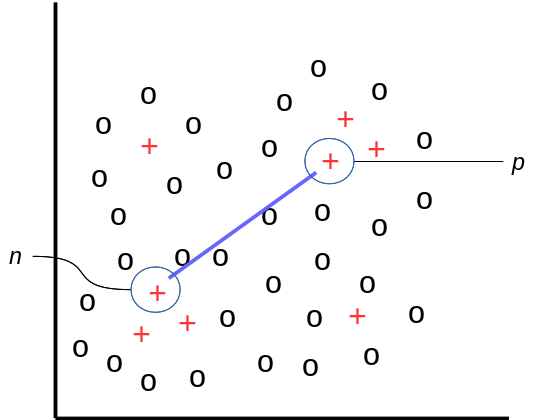
\includegraphics[keepaspectratio=true,scale=0.35]{SMOTE-example}
}
	\caption{
	Ilustrasi pembuatan sampel sintetis pada SMOTE.
	Misalkan $p$ adalah sampel minoritas dan $n$ adalah salah satu dari $k$
	tetangga terdekat dari $p$, maka
	sampel sintetis yang baru akan berada di garis antara $p$ dan $n$.
	}
	\label{fig:smote}
\end{figure}

Sampel sintetis dibuat dengan cara berikut, misalkan $p$ adalah salah satu
sampel minoritas pada dataset $D$,
\pagebreak
\begin{itemize}
	\item Cari $k$ sampel tetangga dari $p$ pada $D$
	\item Untuk setiap sampel tetangga $k$,
	\begin{itemize}
		\item Hitung selisih antara vektor fitur $p$ dengan tetangga $k_{i}$
		\item Kalikan selisih tersebut dengan angka ril acak antara 0 sampai 1,
		dan
		\item simpan hasilnya ke vektor fitur sintentis yang baru.
	\end{itemize}
\end{itemize}

Cara ini membuat sampel secara acak pada segmen garis antara dua fitur yang
terpilih, seperti yang terlihat pada gambar \ref{fig:smote}.
Pendekatan ini secara efektif mendorong wilayah pembelajaran dari kelas
minoritas menjadi lebih besar tanpa menyebabkan \textit{overfitting}.


\section{LNSMOTE}
Meskipun hasil SMOTE dibuktikan bagus dalam makalah Chawla dkk.
\cite{chawla2002smote}, metode ini masih memiliki beberapa kelemahan.
Pertama, cara menentukan sampel minoritas sebagai calon untuk
\textit{over-sampling} bisa bermasalah.
Pada SMOTE, semua sampel dari kelas minoritas digunakan.
Namun, bukan berarti semua sampel tersebut sama bergunanya bagi pembelajaran
klasifikasi.
Pada khususnya, sampel yang ada pada batas \textit{decision}, atau berada
dibatas kelas minoritas dengan kelas mayoritas, lebih sering salah
diklasifikasi dibandingkan dengan sampel yang berada jauh dari batas kelas,
oleh karena itu mereka lebih penting untuk klasifikasi.
Sampel yang jauh dari batas kelas, berada di tengah kelas minoritas mungkin
berkontribusi sedikit pada klasifikasi.
Salah satu metode untuk menangani permasalahan ini yaitu dengan hanya
mengambil sampel pada batas kelas minoritas yang dijadikan untuk
\textit{oversampling}, seperti yang diajukan oleh Han dkk.
\cite{han2005borderline} dengan menggunakan metode bernama \textit{Borderline
SMOTE}.

\begin{figure}[htbp]
	\centering
	\begin{subfigure}[b]{0.4\textwidth}
		\centering
		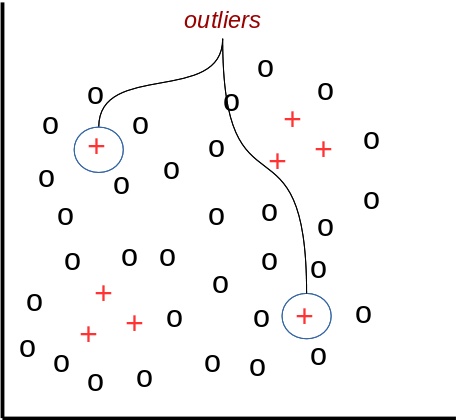
\includegraphics[width=\textwidth]{SMOTE-problem-outliers}
		\caption{}
		\label{fig:smote-outliers}
	\end{subfigure}
	\begin{subfigure}[b]{0.5\textwidth}
		\centering
		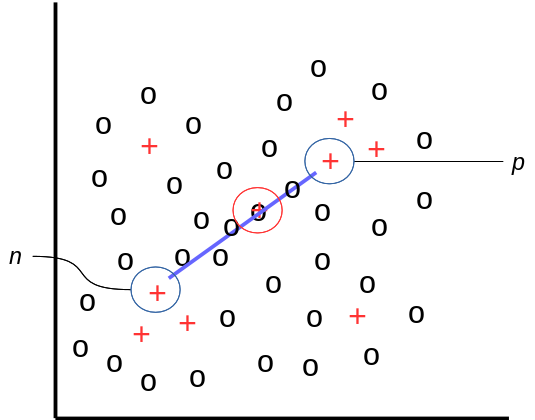
\includegraphics[width=\textwidth]{SMOTE-problem-overlapping}
		\caption{}
		\label{fig:smote-overlapping}
	\end{subfigure}
	\caption{
Kelemahan metode SMOTE:
(a) \textit{Outliers} pada kelas minoritas tidak diperhitungkan pada metode
SMOTE.
(b) Pembuatan sampel sintetis yang baru berada di wilayah kelas mayoritas
yang tumpang-tindih dengan sampel kelas mayoritas.
	}
	\label{fig:smote-problems}
\end{figure}

Kelemahan lain dari SMOTE yaitu permasalahan \textit{overgeneralization} yang
begitu saja menggeneralisasi wilayah dari kelas minoritas.
SMOTE tidak mempertimbangkan distribusi dari sampel pada kelas mayoritas, atau
adanya \textit{outliers}.

Untuk mengatasi permasalahan di atas, Maciejewski dkk. memperkenalkan ekstensi
dari metode SMOTE bernama \textit{Local-neighbourhood SMOTE} atau disingkat
LNSMOTE \cite{maciejewski2011local} yang menggunakan modifikasi dari
pendekatan \textit{Safe-Level SMOTE} \cite{bunkhumpornpat2009safe}.
Pada metode \textit{Safe-level SMOTE} keberadaan sampel mayoritas
diperhitungkan sebelum membuat sampel sintetis dengan menghitung sebuah
koefisien khusus yang disebut \textit{safe level}.
Untuk setiap sampel dari kelas minoritas, dihitung jumlah sampel kelas
minoritas di antara \textit{k-nearest-neighbors} (KNN).
Jika nilainya sama atau mendekati $ 0 $, sampel tersebut dianggap sebagai
\textit{noise}.
Jika nilainya mendekati $ k $, maka sampel tersebut bisa dikatakan berada
di wilayah aman dari kelas minoritas.
Gagasan utamanya adalah membuat sampel sintetis yang dekat dengan wilayah aman.

Lebih rincinya, misalkan $ p $ adalah sampel dari kelas minoritas yang akan
menjadi calon untuk \textit{over-sampling}, maka $ k $ sampel terdekat dengan
$ p $ yang termasuk pada kelas minoritas $ P $ ditentukan.
Seperti pada SMOTE, setidaknya satu dari tetangga tersebut dipilih, sebutlah
dengan $ n $.
Untuk kedua sampel, $ p $ dan $ n $, $ k $ sampel terdekatnya untuk keseluruhan
data pelatihan $ S $ dihitung \textit{safe level}-nya dengan notasi $ sl(p) $
dan $ sl(n) $.
Dari pengetahuan tersebut, koefisien rasio \textit{safe-level} ditentukan
dengan $ \textit{sl-ratio} = sl(p) / sl(n) $.
Langkah selanjutnya ditentukan berdasarkan 5 kasus berikut:
\begin{enumerate}
	\item \label{case:safe-1} Jika $ sl(p) = 0 $ dan $ sl(n) = 0 $, sampel
	$ p $ dan $ n $ dianggap sebagai \textit{noise outliers}, dan tidak ada
	sampel sintetis yang dibuat.
	\item Jika $ sl(p) > 0 $ dan $ sl(n) = 0 $, maka $ n $
	adalah \textit{noise}.
	Sampel sintetis akan dibuat jauh dari $ n $ dengan menduplikasi $ p $.
	\item Jika $ sl-ratio = 1 $, maka $ p $ dan $ n $ memiliki tetangga
	yang sama dan sampel sintetis yang baru akan dibuat diantara garis yang
	menghubungkan mereka dengan cara yang sama seperti pada SMOTE.
	\item Jika $ sl-ratio > 1 $, maka $ p $ berada di wilayah
	aman minoritas daripada $ n $ dan sampel sintetis yang baru akan
	dibuat dekat dengan $ p $, dengan parameter acak pada SMOTE akan
	memiliki rentang $ [0, 1 / \textit{sl-ratio}] $.
	\item Jika \textit{sl-ratio < 1}, maka \textit{n} berada di wilayah
	aman minoritas daripada $ p $ dan sampel sintetis yang baru akan
	dibuat dekat dengan $ n $, yaitu parameter acak pada SMOTE akan
	memiliki rentang $ [1 - \textit{sl-ratio}, 1] $.
\end{enumerate}

Strategi \textit{safe-level SMOTE} bermasalah khususnya pada distribusi kelas
yang bias yang mana kelas minoritas menyebar sehingga terdiri dari beberapa
sub-wilayah dengan kardinalitas yang kecil.
Situasi ini mengacu pada permasalahan yang disebut \textit{small disjuncts}
yang diakui sebagai sumber kesulitan yang paling penting bagi pembelajaran
klasifikasi untuk data timpang \cite{jo2004class}.
Pada kasus seperti ini pembuatan sampel sintetis dengan \textit{Safe-level
SMOTE} bisa menyebabkan terjadinya tumpang-tindih antara kelas.

Sebagai contohnya, misalkan dua kelompok dari kelas minoritas terpisah
dikelilingi oleh sampel dari kelas mayoritas.
Katakanlah, jarak antara kedua kelompok minoritas tersebut cukup jauh, satu
kelompok berada di bawah dan kelompok lainnya di atas.
Misalkan calon dari sebuah sampel berada di kelompok yang dibawah.
Jika parameter $ k $ dari fungsi pencarian KNN lebih besar dari jumlah sampel
kelas minoritas di dalam kelompok tersebut, maka tetangga dari kelas minoritas
selanjutnya akan menjadi sampel dari kelompok yang lain.
Jika rasio \textit{safe-level} dari sampel kedua kelompok sama, sampel sintetis
yang baru bisa dibuat diantara garis yang menggabungkan sampel-sampel dari
kedua kelompok tersebut.
Dengan kata lain, sampel sintetis yang baru bisa berada di wilayah yang dihuni
oleh kelas mayoritas.
Makanya, strategi ini masih memungkinkan terjadinya tumpang-tindih antara
kelas.

Situasi tidak diinginkan seperti di atas disebabkan karena teknik SMOTE mencari
KNN yang dimiliki oleh kelas minoritas saja.
Jika calon sampel tidak berada di wilayah yang padat dengan kelas minoritas,
maka beberapa tetangganya bisa saja cukup jauh dan juga sampel dari kelas
mayoritas mengelilingi calon sampel tersebut.

LNSMOTE mengatasi masalah tumpang tindih ini dengan lebih mempertimbangkan
tetangga sekitar
(\textit{local neighbourhood})
dari calon sampel minoritas yang mungkin bisa memberikan perkiraan dari
keberadaan sampel kelas mayoritas.
Jadi, pencarian sampel yang terlalu jauh sebaiknya dihindarkan.

Modifikasi teknik LNSMOTE terhadap \textit{Safe-Level} SMOTE yaitu,
\begin{itemize}
\item jika calon sampel $ p $ diidentifikasi berada di tetangga terdekat $ k
$ dari $ n $, sampel tersebut tidak langsung dihitung dengan $ sl(n) $ tapi
dicari tetangga dari $ k + 1 $ selanjutnya.
\item Membatasi rentang interval di mana sampel baru secara acak ditempatkan.
Jadi, pada beberapa kasus dari \textit{safe-level}, LNSMOTE tidak menentukan
batas kanan dari interval dengan 1 tapi sebagai ambang batas $\tau < 1$.
Ambang batas tersebut tidak baku tapi ditentukan secara dinamis bergantung
kepada \textit{safe-level} dari sampel mayoritas.
\item Jika $ sl(n) $ relatif rendah, artinya $ n $ dikelilingi oleh banyak
sampel dari kelas mayoritas, sampel baru seharusnya ditempatkan lebih dekat ke
$ p $.
\item Jika $ n $ dikelilingi oleh sejumlah sampel minoritas yang seimbang,
sehingga nilai $ sl(n) $ tinggi, sampel yang baru bisa berada di dekat $ n $.
Hal ini supaya bisa mengontrol tingkat ekspansi dari kelas minoritas dengan
cara dinamis, memperhitungkan distribusi lokal dari sampel.
\end{itemize}

Algoritma LNSMOTE yang digunakan pada implementasi tesis berdasarkan pada
makalah Maciejewski dkk.
\cite{maciejewski2011local}
yang dapat dilihat pada lampiran
\ref{lampiran:alg_lnsmote}.


\section{\textit{Random Forest}}
\textit{Random Forest} (RF) \cite{breiman2001random}
adalah sebuah kombinasi dari beberapa pohon keputusan yang mana setiap pohon
bergantung kepada nilai dari vektor acak yang disampel secara independen dan
dengan distribusi yang sama.

Pohon keputusan yang digunakan dalam RF dapat menggunakan ID3
(\textit{Iterative Dichotomiser}), C4.5 (pengganti dari ID3), atau CART
(\textit{Classification and Regression Trees}).
Dalam tesis ini, dan umumnya pada implementasi RF, menggunakan CART sebagai
pohon keputusan.

Ada tiga parameter utama dalam pembentukan RF.
Parameter pertama yaitu jumlah pohon yang akan dibangun dalam \textit{forest}
(katakanlah $n$),
parameter kedua yaitu persentase dari sampel pelatihan yang digunakan untuk
membangun pohon (katakanlah $b$),
dan parameter ketiga yaitu jumlah fitur acak yang juga digunakan untuk
membangun pohon (katakanlah $m$).
Ketiga parameter diatur sebelum memulai pembangunan RF dan nilainya sama untuk
semua pohon.

Persentase dari sampel pelatihan yang diambil secara acak umumnya dua per tiga
dari sampel keseluruhan, sehingga meninggalkan sepertiganya sebagai
\textit{out-of-bag} (OOB).
Untuk nilai acak fitur $m$, nilai yang biasa digunakan yaitu akar dari jumlah
fitur atau $log$ dari jumlah fitur \cite{breiman2001random}.

Proses pembangunan RF sebagai berikut.
Diasumsikan diberikan sebuah dataset latihan $S$.
Setelah parameter ditentukan, pada saat pembuatan pohon, ambil sampel dari $S$
secara acak tanpa diganti (sampel yang telah diambil bisa terpilih kembali pada
pengambilan acak berikutnya) sejumlah $b$.
Proses ini dikenal juga dengan \textit{bootstraping}.
Sampel yang tidak terpilih disebut dengan \textit{out-of-bag} (OOB), yang
bisa digunakan untuk penghitungan laju galat mis-klasifikasi.
Dari sampel yang terpilih tersebut ambil $m$ buah fitur secara acak, kemudian
bangun pohon dari $m$ fitur dan $b$ sampel acak tersebut tanpa dibersihkan
(\textit{pruning}).
Ulangi proses tersebut sampai pohon ke-$n$.

Proses klasifikasi pada RF berjalan seperti berikut.
Diberikan dataset $T$ yaitu dataset yang berisi fitur yang sama dengan dataset
pelatihan $S$.
Untuk setiap sampel yang akan diklasifikasi pada dataset $T$, masukan sampel
tersebut ke setiap pohon.
Kumpulkan hasil klasifikasi dari setiap pohon, kemudian ambil mayoritas kelas
dari semua hasil klasifikasi tersebut.
Fungsi selengkapnya dari pembuatan dan klasifikasi RF dapat dilihat pada
algoritma \ref{alg:rf}.

\begin{center}
\captionof{algorithm}{Random Forest}
\label{alg:rf}
	\begin{algorithmic}[1]
\Require \\
$ TSET $: dataset pelatihan \\
$ T $: jumlah pohon untuk \textit{forest} \\
$ B $: persentase sampel yang dipilih secara acak tanpa diganti dari $TSET$ \\
$ m $: jumlah fitur acak \\

\Function{RandomForest}{$ TSET, T, B, m $}
	\State $ n \gets $ jumlah sampel pada dataset $ TSET $
	\State $ b \gets n * (B / 100) $
	\Comment Jumlah sampel untuk setiap pohon.

	\State $ forest \gets nil $
	\For{$ t \gets 1,T $}
		\State $ tp, tn, tree \gets \Call{GrowTree}{forest, TSET, b, m} $
		\State $ \Call{forest.Add}{tree} $
	\EndFor
	
	\State \Return $forest$
\EndFunction
\\
\Function{GrowTree}{$ forest, TSET, b, m $}
	\label{bagging}
	\State $ bag, oob, bagIdx, oobIdx \gets \Call{RandomPickSample}{$ TSET,
	b $} $

	\State $ tree \gets \Call{BuildTree}{bag, m} $

	\State $ \Call{forest.SaveBagIndex}{bagIdx} $
	\Comment Simpan pohon dan indeks dari \textit{bagging}

	\State $ cm \gets \Call{Classify}{forest, oob, oobIdx} $
	\State $ tp, tn \gets \Call{ComputeStat}{cm} $
	\Comment Hitung laju galat OOB dari \textit{confusion matrix}
	$cm$.

	\State \Return{$ tp, tn, tree $}
\EndFunction
\\
\Function{Classify}{$ forest, set, setIdx $}
	\State $ predictions \gets nil $
	\For{\textbf{each} $ sample, idx $ \textbf{in} $ set $}
		\State $ votes \gets \Call{ForestVotes}{forest, sample, idx} $
		\State $ class \gets \Call{Majority}{votes} $
		\Comment ambil mayoritas suara kelas pada $votes$
		\State $ predictions.push(class) $
	\EndFor

	\State \Return $predictions$
\EndFunction
\\
\Function{ForestVotes}{$ forest, sample, idx $}
	\State $ votes \gets nil $
	\For{\textbf{each} $ tree $ \textbf{in} $forest$ }
		\State $ exist \gets \Call{IsSampleInTheBag}{idx} $
		\Comment Periksa apakah sampel indeks digunakan pada pohon ini.

		\If{exist}
			\State continue
			\Comment Jika digunakan, lanjutkan ke pohon berikutnya.
		\EndIf

		\State $ class \gets \Call{tree.Classify}{sample} $

		\State $ \Call{votes.push}{class} $
	\EndFor

	\State \Return $ votes $
\EndFunction
	\end{algorithmic}
\end{center}



\section{Cascaded Random Forest}
Permasalahan umum dalam penggalian data atau algoritma pembelajaran ansambel
adalah ketidakmampuan untuk menangani data pelatihan yang timpang.
Ketimpangan antara kelas positif dan negatif biasanya menyebabkan akurasi
deteksi yang rendah.
Simulasi yang dilakukan oleh Strobel dkk. \cite{strobl2007bias} menampilkan
bahwa RF condong mendukung kelas mayoritas.
Saat menggunakan RF untuk deteksi, sejumlah besar sampel negatif dibutuhkan
untuk mendapatkan pengklasifikasi yang kuat dan laju \textit{false-positive}
yang rendah.
Hal ini menyebabkan ketimpangan yang besar antara kelas positif dan
negatif, sehingga membuat pengklasifikasi RF yang berfokus pada kelas
mayoritas.
Kelemahan lain dari RF yaitu setelah belajar dengan beberapa pohon, RF secara
gradual mencapai titik puncaknya, yang mana pengklasifikasi tidak bisa lagi
meningkatkan \textit{sensitivity} pada pendeteksian maupun mengurangi laju
\textit{false-positive}-nya.

Pada tahun 2011, Viola dan Jones mengajukan algoritma deteksi sampel cepat
berbasis AdaBoost dengan struktur kaskade (\textit{cascade})
\cite{viola2004robust}.
Struktur kaskade dimotivasi oleh asumsi bahwa lebih mudah untuk menolak sebuah
sampel yang negatif daripada mencari sampel yang positif.
Viola dan Jones menggabungkan pengklasifikasi yang kuat pada beberapa tingkatan
yang independen dengan kondisi bahwa setiap tingkat dapat menolak sebuah
sampel, sehingga supaya sebuah sampel dapat dianggap positif semua tingkat
harus terlewati.
Disebabkan karena dominasi penolakan pada tahap-tahap awal, waktu komputasi
menjadi berkurang.
Sebagai tambahan, untuk mendapatkan pelatihan yang lebih baik, Viola dan Jones
mengajukan strategi \textit{bootstrap} dengan menghapus sampel yang benar
terklasifikasi negatif setelah pembelajaran dilakukan pada setiap tingkat.
Setelah itu, dataset pelatihan yang berkurang ditambahkan dengan sampel yang
salah diklasifikasi (\textit{false-positive})
\cite{viola2004robust}.

Sebuah pengklasifikasi kaskade terdiri dari sejumlah tingkatan dengan
kompleksitas yang meningkat.
Setiap tingkat minimum memiliki satu pengklasifikasi independen.
Pengklasifikasi ditambahkan ke dalam tingkatan sampai batas nilai
\textit{true-positive} dan \textit{true-negative} tercapai.
Keuntungan dari struktur kaskade yaitu sejumlah besar sampel dapat
didistribusikan diantara tingkatan, berkurangnya nilai \textit{false-positive},
dan berkurangnya waktu komputasi baik pada pelatihan dan klasifikasi.

Baumann menerapkan metoda ini pada RF dan mengajukan \textit{Cascaded Random
Forest} (CRF) yaitu penggabungan dari pengklasifikasi RF dengan struktur
kaskade, yang menyusun beberapa pohon keputusan dalam setiap tingkatan dengan
strategi agregasi \textit{bootstrap}.
Sehingga, pembelajaran pada sampel positif meningkat dan kelemahan dari data
yang timpang terhindari \cite{baumann2013cascaded}.

Pengklasifikasi CRF memiliki enam parameter umum, tiga diantaranya sama dengan
RF yaitu jumlah pohon ($T$), persentase sampel acak untuk \textit{bootstrap},
($b$), dan jumlah fitur acak ($m$).
Tiga parameter lainnya yaitu jumlah tingkatan ($S$), nilai ambang batas
\textit{true-positive} ($maxtp$), dan nilai ambang batas
\textit{true-negative} ($maxtn$).

Strategi \textit{bootstrap} yang digunakan adalah sebagai berikut: setelah
menyelesaikan pembelajaran pada sebuah tingkatan, dataset pelatihan yang berisi
hanya sampel negatif diujikan ke semua tingkatan yang telah dibentuk
sebelumnya dengan tujuan untuk menghapus sampel yang benar bernilai
\textit{true-negative} saja, sehingga dataset pelatihan sebisa mungkin berisi
hanya sampel positif.
Sampel yang terklasifikasi \textit{false-positive} kemudian dimasukan kembali
ke dataset pelatihan untuk dipelajari oleh tingkatan berikutnya.
Fungsi selengkapnya dari CRF dapat dilihat pada algoritma \ref{alg:crf}.

Beberapa tingkatan memiliki akurasi deteksi yang lebih rendah daripada
yang lainnya.
Untuk mengurangi pengaruh tingkatan yang memiliki performansi yang rendah
tersebut, maka dihitung faktor bobot $\alpha$ dari setiap tingkatan dengan
mengeksploitasi rerata harmonik dari \textit{precision} dan \textit{recall},
atau dikenal juga dengan nilai $F_1$ (\textit{fmeasure}),
pada dataset pelatihan.

Nilai $\alpha$ pada setiap tingkatan secara linear dinormalisasi pada rentang 0
dan 1, sehingga bobot dari tingkat yang memiliki performansi yang rendah
berkurang supaya pengaruhnya terhadap mayoritas \textit{voting} juga berkurang.
Proses untuk mendapatkan hasil dari pengklasifikasi CRF diberikan pada gambar
\ref{form:crf}.

\begin{figure}[h]
\[
	y(x) = argmax \left(
			\frac{1}{T \cdot \sum^{S}_{s=1} \alpha_{s} }
			\sum\limits_{s=1}^{S} \alpha_{s}
			\sum\limits^{T}_{t=1} I_{h_{t} (x) = c}
		\right)
\]
\caption{
Formula untuk mendapatkan kelas (\textit{voting}) pada pengklasifikasi CRF
dengan bobot.
}
\label{form:crf}
\end{figure}

Pada gambar \ref{form:crf}, $x$ adalah sampel yang akan diklasifikasi,
$S$ adalah jumlah tingkatan pada struktur kaskade,
$\alpha_{s}$ adalah nilai bobot dari tingkatan,
$T$ adalah jumlah pohon pada tingkatan, dan
$h_{t}$ yaitu fungsi klasifikasi dari sebuah pohon yang memberikan sebuah nilai
kelas $c$ yang bisa memiliki nilai indikator dari $I$
(misalkan nilai 1 untuk positif atau 0 untuk negatif).


Pada bab ini dijelaskan proses dari pengolahan dataset dan implementasi
algoritma sampel ulang dan klasifikasi, dimulai dari persiapan
data, pembuatan dataset fitur, sampel ulang pada dataset fitur, dan
implementasi pengklasifikasi sehingga nantinya dapat digunakan untuk pelatihan,
pengujian dan analisis.


\chapter{Hasil dan Analisis}

Pelatihan model dilakukan dengan cara menjalankan program klasifikasi RF dan
CRF pada masing-masing dataset fitur WVC2010 yang belum disampel ulang, yang
telah disampel ulang dengan SMOTE, dan yang telah disampel ulang dengan
LNSMOTE.
Setelah modelnya terbangun, model diuji dengan diberikan input dataset fitur
WVC2011. Hasil dari pengujian digunakan untuk analisis.

Lingkungan pelatihan dan pengujian dilakukan pada mesin Intel\textregistered\
 Core\texttrademark \ i7-4750HQ CPU 2,00 GHz, dengan jumlah \textit{RAM} 8
GB. Setiap pelatihan model dilakukan satu per satu untuk menghindari adanya
\textit{cache miss} yang berpengaruh pada kecepatan dan waktu pemrosesan.

\section{Dataset}

Dataset yang digunakan untuk pelatihan model yaitu WVC2010 yang terdiri dari
tiga jenis yaitu dataset tanpa sampel ulang, dataset yang telah disampel ulang
dengan SMOTE, dan dataset yang telah disampel ulang dengan LNSMOTE.
Jumlah sampel pada dataset yang tidak disampel yaitu 2394 positif dan 30045
negatif dengan total 32439 sampel.
Jumlah sampel positif pada dataset hasil sampel ulang dengan SMOTE yaitu 28728
sampel dengan total 58773 sampel.
Jumlah sampel positif pada dataset hasil sampel ulang dengan LNSMOTE yaitu
28588 sampel dengan total 58633 sampel.

Dataset yang digunakan untuk pengujian model yaitu WVC2011 yang terdiri dari
1143 sampel positif dan 8842 sampel negatif dengan total 9985 sampel.
Jumlah fitur pada WVC2011 sama dengan WVC2010 yaitu 26 fitur.

\section{Parameter Pelatihan Model}

Supaya konsisten antara pengklasifikasi, digunakan parameter umum yang sama,
seperti jumlah pohon, jumlah fitur acak, dan persentase \textit{bootstrapping};
yaitu 200 pohon, 5 fitur acak, dan $ 64\% $ untuk \textit{bootstrapping}.
Untuk klasifikasi CRF dilakukan tiga pemodelan dan pengujian dengan parameter
yang berbeda yaitu 200 tingkat dengan 1 pohon, 100 tingkat dengan 2 pohon, dan
50 tingkat dengan 4 pohon; dengan jumlah pohon yang tetap sama yaitu 200.
Hal ini dilakukan untuk melihat pengaruh dari jumlah pohon terhadap tingkat dan
hasil klasifikasi.
Parameter lain pada pemodelan CRF yaitu nilai ambang batas TPR dan TNR diset
pada nilai $0,95$ dan $0,95$ untuk mendapatkan hasil klasifikasi yang bagus dan
jumlah pohon yang konsisten.

\section{Hasil Pengujian}

Hasil pengujian diberikan dalam bentuk performansi pengklasifikasi pada tabel
\ref{tab:stats} dan kecepatan pelatihan model pada tabel
\ref{tab:runtimes}.

\DTLsetseparator{;}
\DTLloaddb{stats}{../result/stats.csv}
\DTLmaxforcolumn{stats}{TPR}{\maxtpr}
\DTLminforcolumn{stats}{FPR}{\minfpr}
\DTLmaxforcolumn{stats}{TNR}{\maxtnr}
\DTLmaxforcolumn{stats}{Presisi}{\maxprec}
\DTLmaxforcolumn{stats}{F-Measure}{\maxfm}
\DTLmaxforcolumn{stats}{Akurasi}{\maxacc}
\DTLmaxforcolumn{stats}{AUC}{\maxauc}

\begin{table}[htbp]
\caption{Performansi Klasifikasi RF dan CRF}
\centering
\footnotesize
\begin{tabular}{p{2cm} p{2cm} rrrrrrr}
\hline
\textbf{Klasifikasi} &
\textbf{Dataset} &
\textbf{TPR} &
\textbf{FPR} &
\textbf{TNR} &
\textbf{Pres.} &
\textbf{F-Mea.} &
\textbf{Aku.} &
\textbf{AUC}
\DTLforeach*{stats}{%
	\cl=Klasifikasi,%
	\ds=Dataset,%
	\tpr=TPR,%
	\fpr=FPR,%
	\tnr=TNR,%
	\prec=Presisi,%
	\fm=F-Measure,%
	\acc=Akurasi,%
	\auc=AUC%
}{%
	\DTLifnullorempty{\cl}
		{\\ \cline{2-9}}
		{\\ \hline \hline}
	\DTLifnullorempty{\cl}
		{}
		{
			\multirow{4}{2cm}{\cl}
		}
	& \ds
	& \DTLifnumeq{\tpr}{\maxtpr}{\textbf{\tpr}}{\tpr}
	& \DTLifnumeq{\fpr}{\minfpr}{\textbf{\fpr}}{\fpr}
	& \DTLifnumeq{\tnr}{\maxtnr}{\textbf{\tnr}}{\tnr}
	& \DTLifnumeq{\prec}{\maxprec}{\textbf{\prec}}{\prec}
	& \DTLifnumeq{\fm}{\maxfm}{\textbf{\fm}}{\fm}
	& \DTLifnumeq{\acc}{\maxacc}{\textbf{\acc}}{\acc}
	& \DTLifnumeq{\auc}{\maxauc}{\textbf{\auc}}{\auc}
}
\\
\hline
\end{tabular}
\label{tab:stats}
\end{table}

\DTLloaddb{runtimes}{../result/runtimes.csv}

\begin{table}[htbp]
\caption{Kecepatan pelatihan model}
\centering
\footnotesize
\begin{tabular}{p{4cm} p{4cm} r}
\hline
\textbf{Klasifikasi} &
\textbf{Dataset} &
\textbf{Waktu (menit)}
\DTLforeach*{runtimes}{%
		\cl=Klasifikasi,
		\ds=Dataset,
		\time=Waktu (menit)%
}{%
	\DTLifnullorempty{\cl}
		{\\ \cline{2-3}}
		{\\ \hline \hline}
	\DTLifnullorempty{\cl}
		{}
		{
			\multirow{3}{4cm}{\cl}
		}
	& \ds
	& \time
}
\\
\hline
\end{tabular}
\label{tab:runtimes}
\end{table}

Klasifikasi CRF LNSMOTE dengan 200 tingkat 1 pohon memberikan nilai TPR paling
tinggi yaitu $0,9904$ tapi dengan nilai FPR yang paling tinggi yaitu $0,8558$
dan TNR yang paling rendah yaitu $0,1442$ di antara model yang lainnya.
Kebalikannya, pengklasifikasi RF tanpa sampel ulang memberikan nilai TNR paling
tinggi yaitu $0,9988$ dan nilai FPR paling rendah yaitu $0,0012$.
Untuk presisi, RF tanpa sampel ulang memberikan nilai tertinggi yaitu $0,9450$,
dan nilai terendah diberikan oleh klasifikasi CRF LNSMOTE dengan 200 tingkat 1
pohon.
Untuk nilai \textit{F-Measure}, nilai tertinggi diberikan oleh klasifikasi CRF
tanpa sampel ulang dengan 50 tingkat dan 4 pohon yaitu $0,5353$, dengan nilai
terendah diberikan oleh klasifikasi CRF LNSMOTE 200 tingkat 1 pohon.
Untuk nilai akurasi tertinggi didapat dengan klasifikasi RF LNSMOTE dengan
yang terendah diberikan oleh klasifikasi CRF LNSMOTE 200 tingkat 1 pohon.
Klasifikasi dengan nilai AUC tertinggi yaitu CRF SMOTE 100 tingkat 2 pohon
dengan yang terendah diberikan oleh klasifikasi CRF tanpa sampel ulang dengan
100 tingkat 2 pohon.

Dari segi kecepatan pelatihan model, pengklasifikasi CRF lebih cepat dari RF
baik pada semua dataset pelatihan.
Sebagai pembanding, dapat dilihat pada klasifikasi RF dan CRF 50 tingkat 4
pohon.
CRF tanpa sampel ulang lebih cepat 11 kali daripada RF, dan pada sampel ulang
SMOTE dan LNSMOTE, klasifikasi CRF 1,6 kali lebih cepat daripada RF.

\chapter{Analisis}

Hasil pelatihan dan pengujian model dianalisis dalam tiga bagian.
Pertama, analisis dari metode sampel ulang LNSMOTE, kedua, analisis terhadap
pengklasifikasi CRF, dan yang terakhir yaitu analisis terhadap hasil
keseluruhan.

\section{Analisis Sampel-ulang}

Pengaruh sampel ulang SMOTE dan LNSMOTE berbeda pada klasifikasi RF dan CRF.
Pada klasifikasi RF, sampel ulang dengan LNSMOTE lebih baik dari SMOTE dengan
meningkatnya nilai akurasi $0,4\%$.
Pada klasifikasi CRF, metode SMOTE secara keseluruhan memberikan performansi
lebih baik daripada LNSMOTE dengan nilai AUC tertinggi didapat dengan CRF 100
tingkat 2 pohon.
Perbedaan  sampel ulang dengan SMOTE dan LNSMOTE yaitu meningkatkan nilai
\textit{F-Measure} dan akurasi pada RF, sedangkan pada CRF sebaliknya, seperti
yang terlihat pada kolom \textit{F-Measure} dan akurasi di tabel
\ref{tab:stats}.
Kelemahan dari LNSMOTE yaitu meningkatkan nilai FPR dari
klasifikasi lebih tinggi dari SMOTE, seperti yang terlihat pada kurva ROC pada
gambar \ref{fig:roc} (c) dan (d).

\label{fig:roc}
\begin{figure}[htbp]
\centering
\begin{tikzpicture}
	\pgfplotsset{
		small,
	}
	\matrix{
		\begin{axis}[
			title=(a),
			ylabel=$TPR$,
			legend columns=-1,
			legend entries={Tanpa sampel ulang\ ,SMOTE\ ,LN-SMOTE},
			legend to name=roc_legend
		]
			\addplot table[
				x={FPR},
				y={TPR},
			]
			{../result/rf.csv};
			\addplot table[
				x={FPR},
				y={TPR},
			]
			{../result/rf_smote.csv};
			\addplot table[
				x={FPR},
				y={TPR},
			]
			{../result/rf_lnsmote.csv};
		\end{axis}
		&
		\begin{axis}[
			title=(b),
		]
			\addplot table[
				x={FPR},
				y={TPR},
			]
			{../result/crf_200_1.csv};
			\addplot table[
				x={FPR},
				y={TPR},
			]
			{../result/crf_200_1_smote.csv};
			\addplot table[
				x={FPR},
				y={TPR},
			]
			{../result/crf_200_1_lnsmote.csv};
			title=(b),
		\end{axis}
		\\
		\begin{axis}[
			title=(c),
			xlabel=$FPR$,
			ylabel=$TPR$,
		]
			\addplot table[
				x={FPR},
				y={TPR},
			]
			{../result/crf_100_2.csv};
			\addplot table[
				x={FPR},
				y={TPR},
			]
			{../result/crf_100_2_smote.csv};
			\addplot table[
				x={FPR},
				y={TPR},
			]
			{../result/crf_100_2_lnsmote.csv};
		\end{axis}
		&
		\begin{axis}[
			title=(d),
			xlabel=$FPR$,
		]
			\addplot table[
				x={FPR},
				y={TPR},
			]
			{../result/crf_50_4.csv};
			\addplot table[
				x={FPR},
				y={TPR},
			]
			{../result/crf_50_4_smote.csv};
			\addplot table[
				x={FPR},
				y={TPR},
			]
			{../result/crf_50_4_lnsmote.csv};
		\end{axis}
		\\
	};
\end{tikzpicture}
\ref{roc_legend}
\caption{
Kurva ROC untuk klasifikasi RF dan CRF pada tiga dataset yaitu yang
tanpa sampel ulang, yang disampel ulang dengan SMOTE dan LN-SMOTE.
(a) RF dengan 200 pohon
(b) CRF dengan 200 tingkat 1 pohon
(c) CRF dengan 100 tingkat 2 pohon
(d) CRF dengan 50 tingkat 4 pohon
}
\end{figure}


\section{Analisis CRF}

Fokus dari pengklasifikasi CRF yaitu pada pembelajaran sampel negatif.
Pada setiap tingkatan CRF, model diuji ulang dengan semua sampel negatif, yang
didapat dari proses tingkatan sebelumnya, dan hasil yang negatif dihapus dari
sampel pelatihan dan dijadikan sebagai dataset uji pada tingkatan selanjutnya.
Berbeda dengan RF, yang mana tidak ada sampel yang dihapus saat
pelatihan, CRF membuat dataset yang tadinya condong pada kelas mayoritas
sedikit demi sedikit pada setiap tingkatan menjadi sama.
Sehingga, melakukan sampel ulang pada pengklasifikasi dengan CRF tidak membantu
dalam memperbaiki performansi modelnya, namun membuat akurasi dari model hasil
pelatihan menurun.
Hal ini bisa dilihat pada kurva PR-AUC pada gambar \ref{fig:prauc}.

Pada gambar \ref{fig:prauc} (b), yaitu CRF dengan 200 tingkatan dan 1 pohon,
performansi tanpa sampel ulang lebih baik dari yang lainnya, dengan nilai AUC
$0,8673$, dan performansi yang buruk dari dataset LNSMOTE.
Saat jumlah pohon pada setiap tingkatan dinaikan menjadi 2 (dan jumlah
tingkatan diturunkan menjadi 100 supaya jumlah keseluruhan pohon tetap 200),
sampel ulang SMOTE menghasilkan nilai AUC yang paling tinggi diantara
model lainnya yaitu $0,8694$, sementara LNSMOTE masih dengan performansi yang
paling rendah, seperti yang terlihat pada gambar \ref{fig:prauc} (b).
Pada pengujian terakhir dengan 50 tingkatan dan 4 pohon, nilai AUC tertinggi
memang didapat dari SMOTE, tapi rerata performansi keseluruhan dihasilkan dari
CRF tanpa sampel ulang, dengan nilai \textit{F-Measure} yang paling tinggi
diantara pengujian lainnya yaitu $0,5353$.

\label{fig:prauc}
\begin{figure}[htbp]
\centering
\begin{tikzpicture}
	\pgfplotsset{
		small,
	}
	\matrix{
		\begin{axis}[
			title=(a),
			ylabel=$Precision$,
			legend columns=-1,
			legend entries={Tanpa sampel ulang\ ,SMOTE\ ,LN-SMOTE},
			legend to name=rf_crf_prauc_legend
		]
			\addplot table[
				x={TPR},
				y={PREC},
			]
			{../result/rf.csv};
			\addplot table[
				x={TPR},
				y={PREC},
			]
			{../result/rf_smote.csv};
			\addplot table[
				x={TPR},
				y={PREC},
			]
			{../result/rf_lnsmote.csv};
		\end{axis}
		&
		\begin{axis}[
			title=(b),
		]
			\addplot table[
				x={TPR},
				y={PREC},
			]
			{../result/crf_200_1.csv};
			\addplot table[
				x={TPR},
				y={PREC},
			]
			{../result/crf_200_1_smote.csv};
			\addplot table[
				x={TPR},
				y={PREC},
			]
			{../result/crf_200_1_lnsmote.csv};
			title=(b),
		\end{axis}
		\\
		\begin{axis}[
			title=(c),
			xlabel=$Recall$,
			ylabel=$Precision$,
		]
			\addplot table[
				x={TPR},
				y={PREC},
			]
			{../result/crf_100_2.csv};
			\addplot table[
				x={TPR},
				y={PREC},
			]
			{../result/crf_100_2_smote.csv};
			\addplot table[
				x={TPR},
				y={PREC},
			]
			{../result/crf_100_2_lnsmote.csv};
		\end{axis}
		&
		\begin{axis}[
			title=(d),
			xlabel=$Recall$,
		]
			\addplot table[
				x={TPR},
				y={PREC},
			]
			{../result/crf_50_4.csv};
			\addplot table[
				x={TPR},
				y={PREC},
			]
			{../result/crf_50_4_smote.csv};
			\addplot table[
				x={TPR},
				y={PREC},
			]
			{../result/crf_50_4_lnsmote.csv};
		\end{axis}
		\\
	};
\end{tikzpicture}
\ref{rf_crf_prauc_legend}
\caption{
Kurva PR-AUC untuk klasifikasi RF dan CRF pada tiga dataset yaitu yang
tanpa sampel ulang, yang disampel ulang dengan SMOTE dan LN-SMOTE.
(a) RF dengan 200 pohon
(b) CRF dengan 200 tingkat 1 pohon
(c) CRF dengan 100 tingkat 2 pohon
(d) CRF dengan 50 tingkat 4 pohon
}
\end{figure}


\section{Analisis Pengklasifikasi Vandalisme}

\label{fig:rocpoints}
\begin{figure}[htbp]
\centering
\begin{tikzpicture}[framed]
	\pgfplotsset{
		width=12cm,
		xtick distance=0.1,
		ytick distance=0.1,
	}
	\begin{axis}[
		title=Performansi pengklasifikasi pada ruang ROC,
		xlabel=$FPR$,
		ylabel=$TPR$,
		legend columns=3,
		legend entries={
			RF,
			RF-SMOTE,
			RF-LNSMOTE,
			CRF-200-1,
			CRF-200-1-SMOTE,
			CRF-200-1-LNSMOTE,
			CRF-100-2,
			CRF-100-2-SMOTE,
			CRF-100-2-LNSMOTE,
			CRF-50-4,
			CRF-50-4-SMOTE,
			CRF-50-4-LNSMOTE,
		},
		legend to name=class_legend
	]
		\addplot[
			scatter,
			only marks,
			point meta=explicit symbolic,
			every mark/.append style={
				/tikz/mark size=3pt
			},
			scatter/classes={
				rf-noresampling={
					mark=text,
					text mark=$\Box$
				},
				rf-smote={
					mark=text,
					text mark=$\boxplus$
				},
				rf-lnsmote={
					mark=text,
					text mark=$\boxtimes$
				},
				crf-200-1={
					mark=text,
					text mark=$\triangle$
				},
				crf-200-1-smote={
					mark=text,
					text mark=$\triangleleft$
				},
				crf-200-1-lnsmote={
					mark=text,
					text mark=$\triangleright$
				},
				crf-100-2={
					mark=text,
					text mark=$\medcircle$
				},
				crf-100-2-smote={
					mark=text,
					text mark=$\oplus$
				},
				crf-100-2-lnsmote={
					mark=text,
					text mark=$\otimes$
				},
				crf-50-4={
					mark=text,
					text mark=$\Diamond$
				},
				crf-50-4-smote={
					mark=text,
					text mark=$\diamondplus$
				},
				crf-50-4-lnsmote={
					mark=text,
					text mark=$\diamondtimes$
				}
			},
		]
		table[
			x={FPR},
			y={TPR},
			meta=klasifikasi,
		]
		{../result/cm.csv};

		\addplot[
			gray
		]
		coordinates{
			(0,0)
			(1,1)
		};
		\addplot[
			gray
		]
		coordinates{
			(0,1)
			(1,0)
		};
	\end{axis}
\end{tikzpicture}
\newline
\ref{class_legend}
\newline
\caption{
Titik ROC untuk semua pengklasifikasi dan dataset.
CRF-200-1 yaitu klasifikasi CRF
dengan 200 tingkat dan 1 pohon, CRF-100-2 yaitu klasifikasi CRF dengan 100
tingkat dan 2 pohon, dan CRF-50-4 yaitu klasifikasi CRF dengan 50 tingkat dan 4
pohon.
}
\end{figure}


Untuk lebih mudah membandingkan semua pengklasifikasi, digunakan titik
ROC yang digambarkan pada grafik \ref{fig:rocpoints}.
Pada bagian kiri bawah adalah klasifikasi RF, berurutan dari bawah ke atas
yaitu RF tanpa sampel ulang ($\Box$) dengan nilai TPR $0,165$ dan FPR $0,001$,
RF pada sampel ulang SMOTE ($\boxplus$) dengan nilai TPR $0,207$ dan FPR
$0,004$, dan yang
paling atas adalah RF pada sampel ulang LNSMOTE ($\boxtimes$) dengan nilai TPR
$0,235$ dan FPR $0,005$.
RF memberikan performansi dengan TPR dan FPR yang paling rendah di antara semua
pengklasifikasi.
Sampel ulang SMOTE meningkatkan nilai TPR $0,25$ kali dan FPR 4 kali.
Sampel ulang LNSMOTE meningkatkan nilai TPR $0,4$ kali dan nilai FPR 5 kali.

Klasifikasi CRF 200 tingkat 1 pohon (CRF-200-1) memiliki nilai TPR paling
tinggi, dengan titik ROC berada pada bagian paling atas dari semua klasifikasi.
Berurutan dari kiri ke kanan yaitu CRF-200-1 tanpa sampel ulang ($\triangle$)
dengan TPR $0,966$ dan FPR $0,467$, CRF-200-1 SMOTE ($\triangleleft$) di tengah
dengan TPR $0,979$ dan FPR $0,63$, dan CRF-200-1 LNSMOTE ($\triangleright$)
pada ujung kanan dengan TPR $0,99$ dan FPR $0,855$.
Pengklasifikasi CRF-200-1 akan mengembalikan kelas sampel positif dengan benar
tetapi dengan galat yang juga tinggi.
Bisa dilihat juga pengaruh SMOTE dan LNSMOTE terhadap nilai FPR.
Sampel ulang SMOTE memberi pengaruh kenaikan TPR $0,1$ dan $0,4$ untuk FPR dari
dataset awal.
Sampel ulang LNSMOTE meningkatkan TPR $0,3$ dan FPR $0,8$.

Klasifikasi CRF 100 tingkat dengan 2 pohon (CRF-100-2) berada pada bagian atas
tengah dari ROC, yang ditandai dengan marka bulat.
CRF-100-2 tanpa sampel ulang ($\medcircle$) berada paling bawah dan kiri dengan
nilai TPR $0,812$ dan FPR $0,24$.
CRF-100-2 SMOTE ($\oplus$) berada di tengah dengan nilai AUC paling tinggi
dengan TPR $0,903$ dan FRP $0,3603$.
CRF-100-2 LNSMOTE ($\otimes$) dengan TPR paling tinggi dari keduanya yaitu TPR
$0,953$ dan FPR $0,585$.
Sampel ulang SMOTE meningkatkan TPR $0,11$ kali dan FPR $0,5$ kali.
Sampel ulang LNSMOTE meningkatkan TPR $0,17$ dan FPR $1,4$ kali.

Klasifikasi CRF 50 tingkat dengan 4 pohon (CRF-50-4) berada pada bagian tengah
kiri atas pada ROC, yang ditandai dengan marka wajik.
CRF-50-4 tanpa sampel ulang ($\Diamond$) menghasilkan nilai TPR $0,607$ dan FPR
$0,08$.
CRF-50-4 dengan sampel ulang ($\diamondplus$) SMOTE meningkatkan nilai TPR
menjadi $0,783$ dan meningkatkan nilai FPR menjadi $0,223$.
CRF-50-4 dengan sampel ulang LNSMOTE ($\diamondtimes$) meningkatan nilai TPR
menjadi $0,895$ dan juga meningkatkan nilai FPR menjadi $0,388$.
Sampel ulang dengan SMOTE meningkatkan nilai TPR $0,3$ kali dan FPR $1,75$
kali.
Sampel ulang dengan LNSMOTE meningkatkan nilai TPR $0,48$ kali dan FPR $3,75$.



\chapter{Kesimpulan}

Secara keseluruhan, performansi dari sampel ulang LNSMOTE lebih baik daripada
SMOTE untuk kedua pengklasifikasi.
Pengaruh menarik lainnya yaitu pada pengklasifikasi CRF, dengan menggunakan
jumlah pohon lebih sedikit pada setiap tingkatan menghasilkan performansi yang
hampir sama dengan melakukan sampel ulang pada dataset asli, seperti yang
terlihat pada performansi CRF 100 tingkat 2 pohon pada dataset tanpa sampel
ulang, hampir sama dengan CRF 50 tingkat 4 pohon dengan sampel ulang SMOTE.

Untuk model klasifikasi vandalisme yang terbaik tanpa sampel ulang dihasilkan
dari pengklasifikasi CRF dengan 200 tingkat dan 1 pohon dengan nilai TPR
$0,9668$,
untuk model terbaik pada dataset yang telah disampel ulang dengan SMOTE yaitu
CRF dengan 200 tingkat dan 1 pohon dengan nilai TPR $0,9790$,
dan untuk model terbaik dari sampel ulang LNSMOTE yaitu CRF dengan 200 tingkat
1 pohon dengan nilai TPR $0.9904$.
Secara keseluruhan model terbaik yaitu dari CRF 200 tingkat dan 1 pohon yang
telah disampel ulang dengan LNSMOTE.
Selain performansi yang lebih baik, pengklasifikasi CRF juga lebih cepat $1,6$
kali dalam pembentukan model daripada RF pada dataset yang telah disampel
ulang.

\section{Kontribusi}

Kontribusi dari karya tulis ini selain membantu menemukan pengklasifikasi yang
lebih baik dalam mendeteksi vandalisme juga memberikan kerangka kerja untuk
menciptakan dan mengembangkan fitur vandalisme dari dataset mentah tanpa harus
mulai dari awal untuk dapat digunakan dalam penelitian selanjutnya atau
digunakan langsung pada kasus asli. Selain itu juga menyediakan pustaka program
untuk pengolahan data dan fungsi pembelajaran mesin terutama untuk sampel ulang
LNSMOTE dan pengklasifikasi
\textit{Cascaded Random Forest} yang belum ada implementasi secara terbuka pada
program terkenal seperti \textit{Weka}, \textit{Scikit-Learn}, atau \textit{R}.

\section{Pekerjaan Selanjutnya}

Jumlah artikel Bahasa Indonesia di Wikipedia setiap tahun semakin meningkat
seiring dengan bertambahnya jumlah pengguna internet di Indonesia.
Semakin banyak pengguna, kemungkinan vandalisme juga semakin tinggi.
Untuk mengatasi masalah vandalisme tersebut lebih awal, akan lebih baik bila
disiapkan sebuah sistem untuk mendeteksi vandalisme pada Wikipedia
Bahasa Indonesia.
Langkah awalnya bisa dengan mengumpulkan data artikel yang telah dianotasi
dengan vandal, supaya dapat dianalisis untuk pembuatan fitur dan pembuatan
model deteksi vandalisme pada Wikipedia Bahasa Indonesia.

Semua pelatihan model dalam karya tulis ini masih menggunakan algoritma
pengklasifikasi RF dan CRF dalam bentuk serial, yang mana satu pohon dibangun
satu per satu bergantian atau pada saat klasifikasi setiap sampel dimasukan ke
dalam pohon secara bergantian untuk mendapatkan kelasnya.
Penggunaan algoritma paralel, seperti dalam pembentukan dua atau empat pohon
bersamaan dan klasifikasi sampel (pengumpulan kelas di setiap pohon)
bersamaan, bisa membantu mempercepat pelatihan, pengujian dan hasil
klasifikasi.
Pada domain pembelajaran mesin, hal menarik yaitu adanya algoritma
\textit{eXtreme Gradient Boostring} (XGBoost)
\parencite{chen2016xgboost}
yang
mungkin bisa meningkatkan deteksi vandalisme.


\clearpage
\addcontentsline{toc}{section}{DAFTAR PUSTAKA}
\printbibliography

\titleformat{\chapter}[hang]
{\bfseries\large\centering}
{Lampiran \thechapter}
{1em}
{}

\appendix
\chapter{Algoritma LN-SMOTE}
\label{lampiran:alg_lnsmote}
\begin{center}
	\captionof{algorithm}{Local Neighbourhood SMOTE}
	\label{alg:lnsmote}
	\begin{algorithmic}[1]
\Require \\
$ D $: dataset sampel keseluruhan \\
$ minor $: kelas minoritas pada dataset $D$ \\
$ o $: persentase jumlah sampel sintetis yang akan dibuat \\
$ k $: jumlah tetangga terdekat dari sampel yang akan dibuat
\\
\Function{LNSMOTE}{$ D, P, o, k $}
	\State $ S \gets [] $
	\Comment Penampung untuk semua sampel sintetis yang akan dibuat.
	\State $ nsyn \gets o/100 $
	\Comment Jumlah sampel sintetis yang akan dibuat.
	\State $ P \gets $ semua sampel minoritas $minor$ pada dataset $D$.
	\\
	\For{\textbf{each} $ sample $ \textbf{in} $ P $}
		\State $ neighbours \gets \Call{FindNeighbours}{D, sample, k} $
		\For{$ i \gets 1,nsyn $}
			\State $ s \gets \Call{CreateSynthetic}{D, sample, neighbours} $

			\If{$ s \not= nil $}
				\State $ \Call{S.Push}{s} $
			\EndIf
		\EndFor
	\EndFor
	\\
	\State \Return{S}
\EndFunction
\\
\Function{CreateSynthetic}{$ D, sample, neighbors $}
	\State $ neighbor \gets \Call{RandomPick}{neighbors} $
	\If{$ \Call{CanCreate}{D, sample, neighbor} = false $}
		\State \Return nil
	\EndIf
	\\
	\State $ lenAttr \gets \Call{LengthAttribute}{sample} $
	\Comment Simpan jumlah atribut dari sampel.

	\State $ newsample \gets [] $
	\Comment Penampung untuk sampel sintetis yang baru.
	\\
	\For{$ x \gets 1,lenAttr $}
		\If{y \textbf{is} classAttribute}
			\State continue
		\EndIf

		\State $ gap \gets \Call{RandomGap}{D, sample, neighbor, k} $

		\State $ sattr \gets sample.\Call{AttributeAt}{y} $
		\State $ nattr \gets neighbor.\Call{AttributeAt}{y} $
		\State $ diff \gets sattr - nattr $
		\State $ newAttr \gets sattr + (gap \times diff) $

		\State $ newsample.\Call{PushAttribute}{newAttr} $
	\EndFor
	\\
	\State \Return{$ newsample $}
\EndFunction
\\
\Function{CanCreate}{$ D, sample, neighbour $}
	\State $ slp \gets \Call{SafeLevel}{D, sample, k} $
	\State $ sln \gets \Call{SafeLevel2}{D, sample, neighbor, k} $
	\State \Return{$ slp \not= 0 $ \textbf{or} $ sln \not= 0 $}
\EndFunction
\\
\Function{SafeLevel}{$ D, p, k $}
	\State $ pneighbor \gets \Call{FindNeighbours}{ D, p, k } $
	\State \Return{$ pneighbor $ yang kelasnya minoritas}
\EndFunction
\\
\Function{SafeLevel2}{$ D, p, n, k $}
	\State $ nneighbours \gets \Call{FindNeighbours}{ D, n, k } $
	\If{$\Call{Class}{n} \not= minor $ \textbf{and} $ p \in nneighbours $}
		\State Ganti $ p $ di $ nneighbours $ dengan tetanggga $ k + 1 $
		dari $ n $
	\EndIf
	\State \Return{$ nneighbours $ yang kelasnya minoritas}
\EndFunction
\\
\Function{RandomGap}{$ D, p, n, k $}
	\State $ slp \gets \Call{SafeLevel}{D, p, k} $
	\State $ sln \gets \Call{SafeLevel}{D, p, n, k} $
	\State $ \delta \gets 0 $

	\If{$ sln = 0 $ \textbf{and} $ slp > 0 $}
		\State \Return{$ \delta $}
	\EndIf
	\\
	\State $ slratio \gets slp / sln $
	\If{$ slratio = 1 $}
		\State $ \delta \gets \Call{Random}{1} $
	\ElsIf{$ slratio > 1 $}
		\State $ \delta \gets \Call{Random}{1 / slratio} $
	\Else
		\State $ \delta = 1 - \Call{Random}{slratio} $
	\EndIf
\pagebreak
	\If{$ \Call{Class}{n} \not= minor $}
		\State $ \delta = \delta \times (sln / k) $
	\EndIf
	\\
	\State \Return{$ \delta $}
\EndFunction
	\end{algorithmic}
\end{center}


\chapter{Algoritma Random Forest}
\label{lampiran:alg_rf}
\begin{center}
\captionof{algorithm}{Random Forest}
\label{alg:rf}
	\begin{algorithmic}[1]
\Require \\
$ TSET $: dataset pelatihan \\
$ T $: jumlah pohon untuk \textit{forest} \\
$ B $: persentase sampel yang dipilih secara acak tanpa diganti dari $TSET$ \\
$ m $: jumlah fitur acak \\

\Function{RandomForest}{$ TSET, T, B, m $}
	\State $ n \gets $ jumlah sampel pada dataset $ TSET $
	\State $ b \gets n * (B / 100) $
	\Comment Jumlah sampel untuk setiap pohon.

	\State $ forest \gets nil $
	\For{$ t \gets 1,T $}
		\State $ tp, tn, tree \gets \Call{GrowTree}{forest, TSET, b, m} $
		\State $ \Call{forest.Add}{tree} $
	\EndFor
	
	\State \Return $forest$
\EndFunction
\\
\Function{GrowTree}{$ forest, TSET, b, m $}
	\label{bagging}
	\State $ bag, oob, bagIdx, oobIdx \gets \Call{RandomPickSample}{$ TSET,
	b $} $

	\State $ tree \gets \Call{BuildTree}{bag, m} $

	\State $ \Call{forest.SaveBagIndex}{bagIdx} $
	\Comment Simpan pohon dan indeks dari \textit{bagging}

	\State $ cm \gets \Call{Classify}{forest, oob, oobIdx} $
	\State $ tp, tn \gets \Call{ComputeStat}{cm} $
	\Comment Hitung laju galat OOB dari \textit{confusion matrix}
	$cm$.

	\State \Return{$ tp, tn, tree $}
\EndFunction
\\
\Function{Classify}{$ forest, set, setIdx $}
	\State $ predictions \gets nil $
	\For{\textbf{each} $ sample, idx $ \textbf{in} $ set $}
		\State $ votes \gets \Call{ForestVotes}{forest, sample, idx} $
		\State $ class \gets \Call{Majority}{votes} $
		\Comment ambil mayoritas suara kelas pada $votes$
		\State $ predictions.push(class) $
	\EndFor

	\State \Return $predictions$
\EndFunction
\\
\Function{ForestVotes}{$ forest, sample, idx $}
	\State $ votes \gets nil $
	\For{\textbf{each} $ tree $ \textbf{in} $forest$ }
		\State $ exist \gets \Call{IsSampleInTheBag}{idx} $
		\Comment Periksa apakah sampel indeks digunakan pada pohon ini.

		\If{exist}
			\State continue
			\Comment Jika digunakan, lanjutkan ke pohon berikutnya.
		\EndIf

		\State $ class \gets \Call{tree.Classify}{sample} $

		\State $ \Call{votes.push}{class} $
	\EndFor

	\State \Return $ votes $
\EndFunction
	\end{algorithmic}
\end{center}


\chapter{Algoritma Cascaded Random Forest}
\label{lampiran:alg_crf}
\begin{center}
	\captionof{algorithm}{Cascaded Random Forest}
	\label{alg:crf}
	\begin{algorithmic}[1]
\Require \\
$ TSET $: dataset pelatihan \\
$ S $: jumlah tingkatan \\
$ T $: jumlah pohon untuk setiap tingkatan \\
$ B $: persentase sampel yang dipilih secara acak tanpa diganti dari $TSET$ \\
$ m $: jumlah fitur acak \\
$ maxtp $: ambang batas untuk nilai \textit{true-positive} \\
$ maxtn $: ambang batas untuk nilai \textit{true-negative}
\\
\Function{CascadedRandomForest}{$ TSET, S, T, B, m, maxtp, maxtn $}
	\State $ n \gets $ jumlah sampel pada dataset $ TSET $
	\State $ b \gets n * (B / 100) $
	\Comment Jumlah sampel acak untuk setiap pohon.

	\State $ TNSET \gets nil $
	\Comment Penampung untuk sampel \textit{true-negative}.

	\State $ crf \gets nil $
	\Comment Pengklasifikasi yang berisi tingkatan.

	\For{$ s \gets 1,S $}
		\State $ forest \gets nil $

		\For{$ t \gets 1,T $}
			\State $ tp, tn, tree \gets \Call{GrowTree}{forest, S, b, m} $
			\If{$ tp > maxtp $ \textbf{and} $ tn > maxtn $}
				\State Tingkatan selesai
			\Else
				\State $ forest.\Call{Add}{tree} $
			\EndIf
		\EndFor
		\\
		\State $w \gets exp(\Call{FMeasure}{tree}) $
		\Comment Simpan nilai \textit{F-Measure} dari pohon terakhir sebagai
		bobot dari tingkatan.
		\State $ crf.\Call{Add}{forest, w} $
		\Comment Simpan forest dan bobot dari tingkatan.
		\If{$ s = 1 $}
			\State Pindahkan sampel \textit{true-negative} dari
			$TSET$ ke $TNSET$
		\Else
			\State Uji tingkatan sebelumnya dengan $TNSET$
			\State Hapus sampel \textit{true-negative} dari TNSET
			\State Isi ulang $TSET$ dengan sampel
			\textit{false-positive} dari hasil uji $TNSET$
		\EndIf
	\EndFor

	\State \Return{crf}
\EndFunction
\\
\Function{Classify}{$ crf, set $}
	\State $ predictions \gets nil $
	\Comment Penampung untuk prediksi klasifikasi dari $set$.
	\State $ sumw \gets $ Jumlah semua bobot tingkatan dalam $crf$.

	\For{\textbf{each} $sample$ \textbf{in} $set$}
		\State $ stageProbs \gets nil $
		\Comment Penampung untuk probabilitas kelas dari setiap $forest$.

		\For{\textbf{each} $forest$, $w$ \textbf{in} $crf$}
			\State $ votes \gets \Call{Classify}{forest, set, nil} $
			\State $ cwprobs \gets $
				(probabilitas setiap kelas dalam $votes \times w$) /
				($ sumw ~ \times $ jumlah pohon dalam $forest$)
			\State $ stageProbs.\Call{Push}{cwprobs} $
		\EndFor

		\State $ class \gets $ Pilih kelas dengan probabilitas maksimum pada $stageProbs$
		\State $ predictions.\Call{Push}{class} $
	\EndFor
	\\
	\State \Return{predictions}
\EndFunction
	\end{algorithmic}
\end{center}


\end{document}
